
\section{Results}
\label{sec_results}
\subsection{Metrics}
\label{sec_matrics}

In order to answer RQ1 and RQ2, we collect the non-dominated set of solutions from each algorithm for 20 runs, and report it in an attainment-surface as introduced by Fonseca \cite{attainment_surface:1996}. To quantitatively compare the quality of each algorithm, we calculate Hypervolume and Contribution indicators to assess multi-objective Pareto Front.

\textbf{Hypervolume}: The Hypervolume indicator \cite{797969} denotes the space dominated by any of the solutions on the Pareto Front. It is calculated as the hypervolume of the union of hypercubes dominated by each solution on the Front. The bigger the Hypervolume is, the more area is donimated by the Pareto Front in the objective space.

\textbf{Contribution}: Since there is no way to know the true Pareto Front, we use the non-dominated set of joint solutions from all experiments to approximate the true Pareto Front. In this case, the Contribution indicator represents the ratio of solutions on the true Pareto Front are found by a given algorithm.

%\textbf{Diversity}: We are also interested in how the solutions found by a given algorithm spread over the Pareto Front. Intuitively, we would like the solutions to be uniformly distributed. The Diversity indicator introduced by Deb \cite{996017} is used.

To facilitate a more easy comparison across subject programs, all objectives are normalised to the original performance of each subject.

\subsection{Answers to RQs}
\label{sec_answers}

\newcommand{\shallow}{Sha}
\newcommand{\all}{All}
\newcommand{\randomsearch}{Rand}
\newcommand{\nsgaii}{NSGA}
\newcommand{\sr}{\emph{\shallow\randomsearch}}
\newcommand{\sn}{\emph{\shallow\nsgaii}}
\newcommand{\dr}{\emph{\all\randomsearch}}
\newcommand{\dn}{\emph{\all\nsgaii}}

For brevity we use \emph{\shallow} to refer to shallow parameters and \emph{\all} to refer to all parameters including shallow and deep parameters, followed by \emph{\randomsearch} or \emph{\nsgaii} to indicate the search method used (random search or NSGA II). For example, \sn{} refers to using NSGA II to search for better values for shallow parameters.
%In subsequent graphs, the performance of the original program always locates at (1, 1) since all the performance is normalised to it.

\begin{figure*}[htb]
	\centering
	\subfigure[espresso]{
		\label{fig_attainment_espresso}
		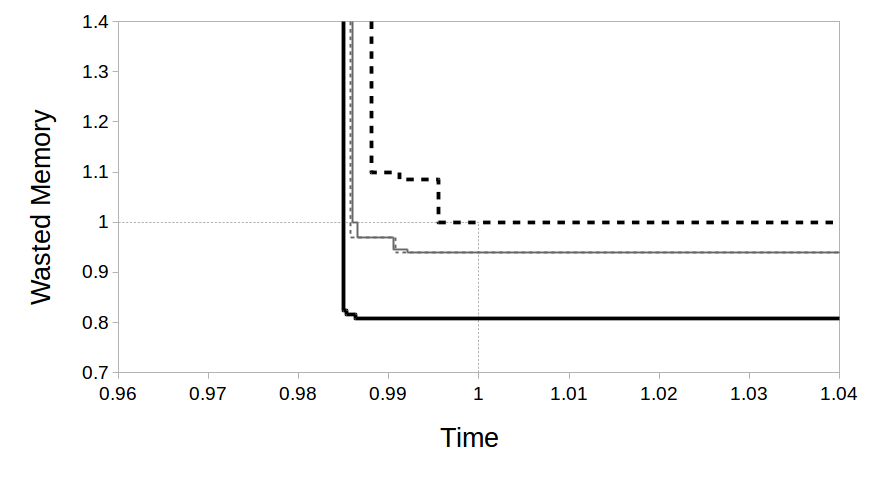
\includegraphics[width=0.47\textwidth]{espresso_attainment_best}%espresso_shallow_random}
	}
	\subfigure[gawk]{
		\label{fig_attainment_gawk}
		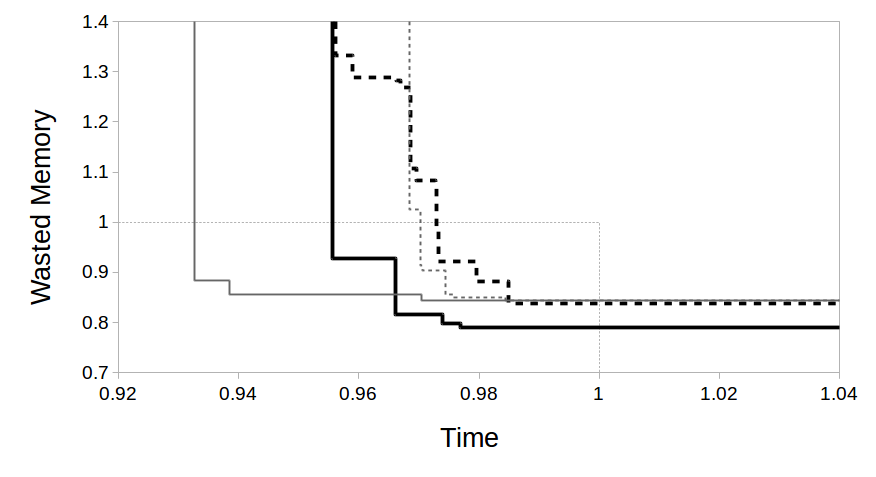
\includegraphics[width=0.47\textwidth]{gawk_attainment_best}%gawk_shallow_random}
	}
	\subfigure[flex]{
		\label{fig_attainment_flex}
		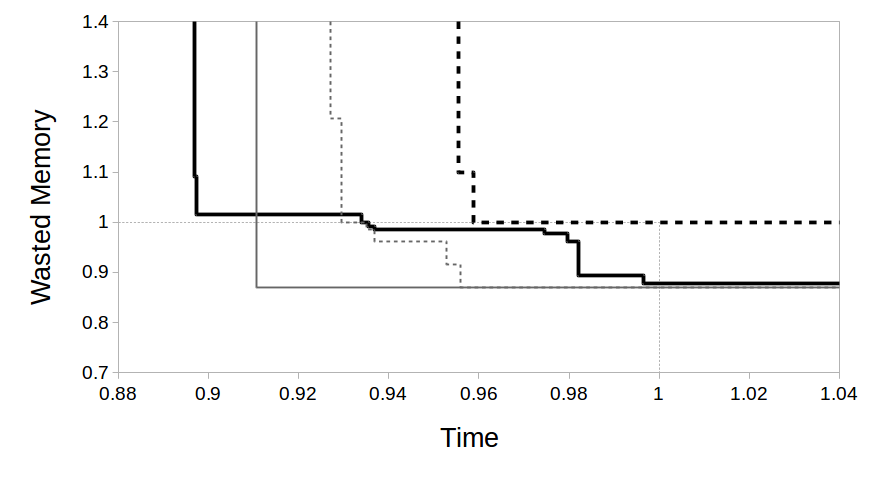
\includegraphics[width=0.47\textwidth]{flex_attainment_best}%flex_shallow_random}
	}
	\subfigure[sed]{
		\label{fig_attainment_sed}
		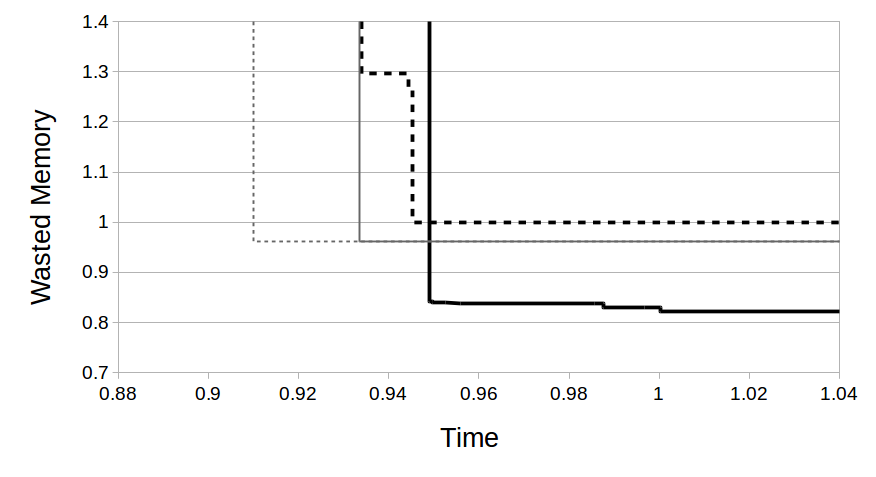
\includegraphics[width=0.47\textwidth]{sed_attainment_best}%sed_shallow_random}
	}
	\subfigure{
		\label{fig_attainment_legend}
		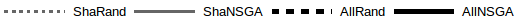
\includegraphics[width=0.5\textwidth]{attainment_legend_best}
	}
	\caption{0\%, 50\%, 100\%-attainment surfaces of the results of \sr{}, \sn{}, \dr{}, \dn{} over 20 runs for each application.}\label{fig_attainment}
\end{figure*}

In order to answer RQ1 and RQ2, we first report the 0\%-attainment surfaces (the combined best solutions over all runs) of the results of \sr{}, \sn{}, \dr{} and \dn{} on all subjects in Figure \ref{fig_attainment}. The solutions are plotted according to their execution time and wasted memory at the high-water-mark compared to the original performance, specially, the original always lies at (1, 1) thus not plotted in the figure. The wasted memory at the high-water-mark is our primary target since the remaining non-wasted memory is needed and thus cannot be reduced. 
In the figure, it is clear that all of the algorithms can reduce time/memory consumption without losing the other performance, implying that the default configuration of \emph{dlmalloc} is not optimal for each application. In three subjects (\emph{espresso}, \emph{gawk} and \emph{sed}), \dn{} outperforms the other three on memory objective. But on time aspect, it's not clear which algorithm is better since different algorithms has their own strengths on different subjects. 
%In Figure \ref{fig_shallow_random}, we can see that Shallow algorithm is better than Random on subject \emph{sed}, while they are incomparable on the other three subjects. In Figure \ref{fig_deep_shallow}, Deep algorithm is better than Shallow on three out of four subjects: \emph{espresso}, \emph{gawk}, \emph{sed}, while incomparable on subject \emph{flex}. Notice that unlike other three subjects, Deep can not find solutions have better performance on memory consumption on subject \emph{flex}, and both Shallow and Deep algorithm perform as good as Random, it implies that the optimal solution is very easy to find in the search space. So any search algorithm would fail to ourperform Random search on this special case.

To get a closer look of the results, we calculated the Hypervolume and Contribution indicator of each algorithm on every subject, and report them in Figure \ref{fig_hypervolume} and \ref{fig_contribution} respectively in the means of boxplots for all 20 runs. 
In Figure \ref{fig_hypervolume}, all the values are normalised to the hypervolume of the `true' Pareto Front (combined non-dominating solutions from all experiments), and the closer the value is to 1 the better. It is clear that \dn{} ourperforms the others on subject \emph{espresso} and \emph{sed} while it doesn't perform very well on subject \emph{flex}, and on subject \emph{gawk} the best value reached by \dn{} is better than that of the others.
%In terms of Hypervolume indicator, Deep algorithm performs the best in general, with an exception on subject \emph{flex}. Shallow algorithm is statistically better than Random on subject \emph{sed}, but there is no significant difference between them on the other three subjects. 
In terms of Contribution indicator, the performance of all algorithms are similar to that of Hypervolume Indicator. We still have \dn{} no worse than other algorithms on all subjects but \emph{flex}, on which \sn{} has the biggest Contribution value.
%At last, Figure \ref{fig_diversity} shows that, all three algorithms generate non-dominated solutions with almost the same diversity, with Shallow performs slightly better on subject \emph{flex}.

%Besides the indicators above, we are also interested in the capability of finding extreme solutions of all algorithms. This can be shown by comparing the most time-saving and memory-saving performance found by each of the algorithms. We gather the best performance in terms of time and memory respectively from all 30 runs and show how often these values can be achieved by each of the algorithms in Figure \ref{fig_best_time} and \ref{fig_best_memory}. In terms of time consumption, while incomparable on three subjects, Shallow and Deep consistantly find better performance on subject \emph{sed} than that found by Random, but there is no statistical difference between Shallow and Deep on all subjects. On the other hand, Deep algorithm is able to find more memory reduction on three out of four subjects, indicating the Deep parameters almost always carry extra information on memory usage.

Since \dn{} is good at finding better performance on memory consumption, we report the most memory-saving performance found by each algorithm of each of 20 runs in Figure \ref{fig_best_memory}. On subject \emph{espresso} and \emph{sed}, \dn{} almost guarantees to find more memory reduction than that found by other approaches. On \emph{gawk}, it doesn't find better configurations in terms of memory consumptoin but has the potential to do so.

In all experiments of \dr{} we observe a lot of invalid configurations, which cause the program crash, generated and evaluated.
Unlike shallow parameters, deep parameters are exposed from internal sub-expressions that were not monitored or protected by the programmers, hence they are expected to cause crashes more often. As a result, the valid configurations are diluted in the search space. Without any guidance, \dr{} finds valid configurations less often than \sr{}, thus performs worse than \sr{}. This is also the reason why the performance of \dn{} is not alway stable on all subjects. Despite diluted search space, deep parameters still carry extra information, which allows \dn{} to find better configurations than the ones can be possibly found by \sn{}.
 
\begin{figure}[htbp]
	\centering
	\subfigure[espresso]{
		\label{fig_hypervolume_espresso}
		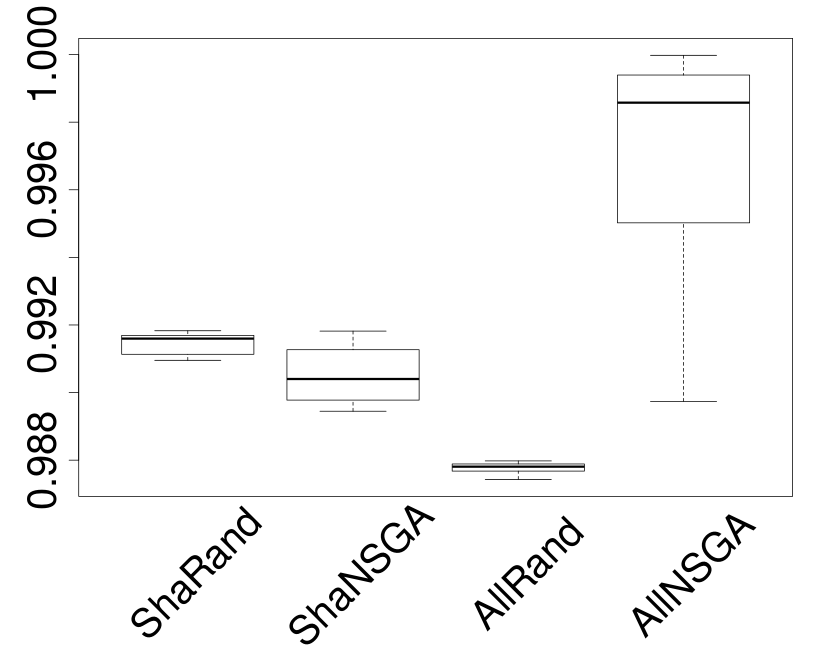
\includegraphics[width=0.22\textwidth]{espresso_hypervolume}
	}
	\subfigure[gawk]{
		\label{fig_hypervolume_gawk}
		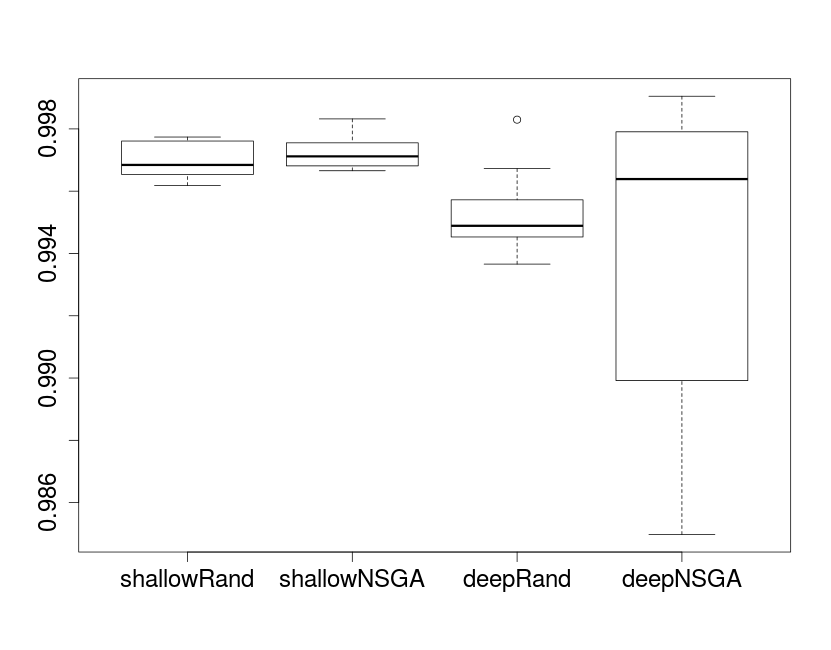
\includegraphics[width=0.22\textwidth]{gawk_hypervolume}
	}
	\subfigure[flex]{
		\label{fig_hypervolume_flex}
		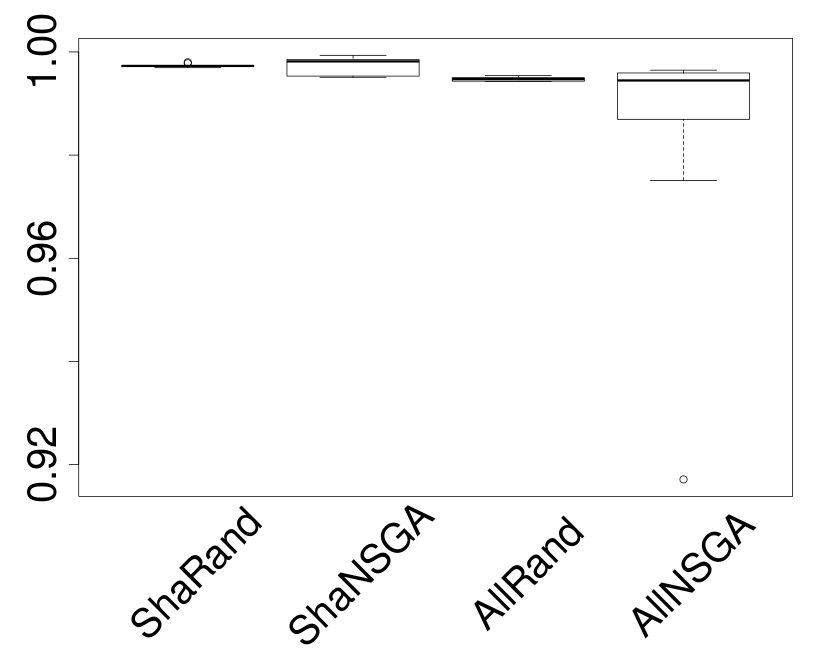
\includegraphics[width=0.22\textwidth]{flex_hypervolume}
	}
	\subfigure[sed]{
		\label{fig_hypervolume_sed}
		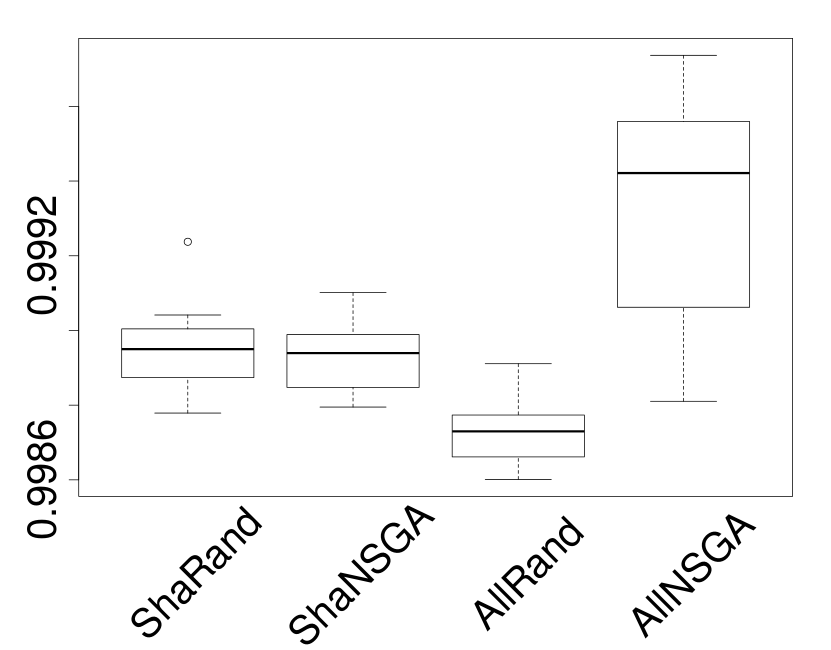
\includegraphics[width=0.22\textwidth]{sed_hypervolume}
	}
	\caption{Hypervolume indicator of \sr{}, \sn{}, \dr{}, \dn{} on all subjects. The values are normalised to the hypervolume of the `true' Pareto Front. Bigger value is better.}\label{fig_hypervolume}
\end{figure}

\begin{figure}[htbp]
	\centering
	\subfigure[espresso]{
		\label{fig_contribution_espresso}
		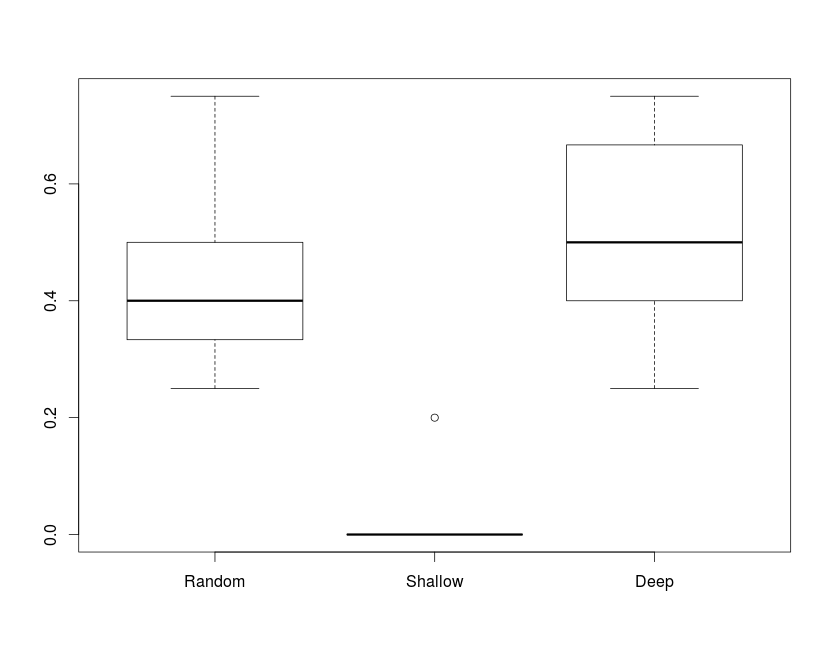
\includegraphics[width=0.22\textwidth]{espresso_contribution}
	}
	\subfigure[gawk]{
		\label{fig_contribution_gawk}
		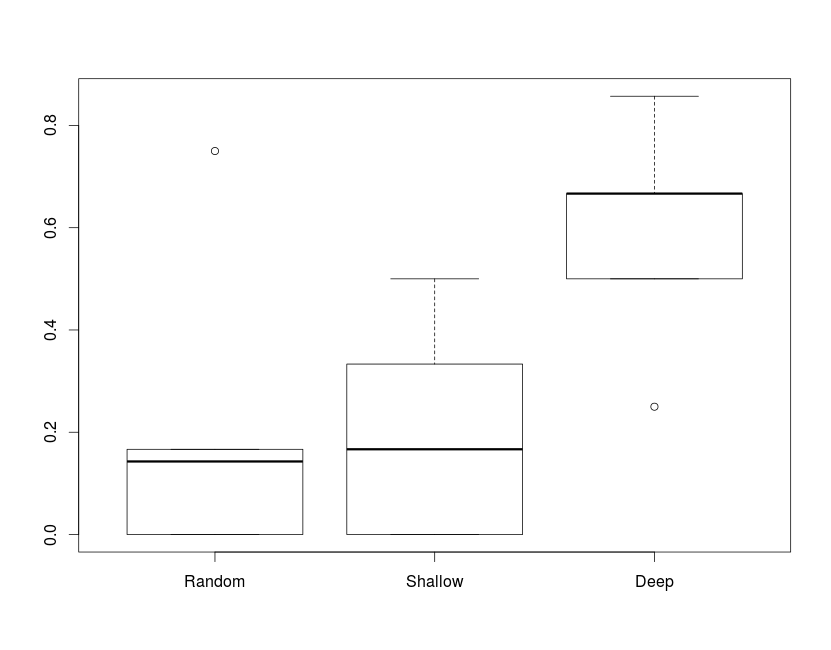
\includegraphics[width=0.22\textwidth]{gawk_contribution}
	}
	\subfigure[flex]{
		\label{fig_contribution_flex}
		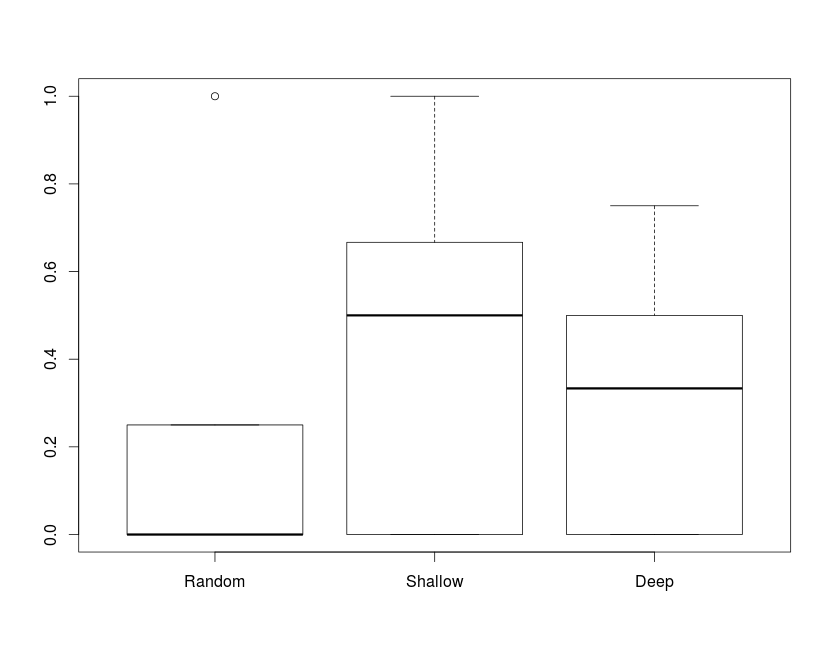
\includegraphics[width=0.22\textwidth]{flex_contribution}
	}
	\subfigure[sed]{
		\label{fig_contribution_sed}
		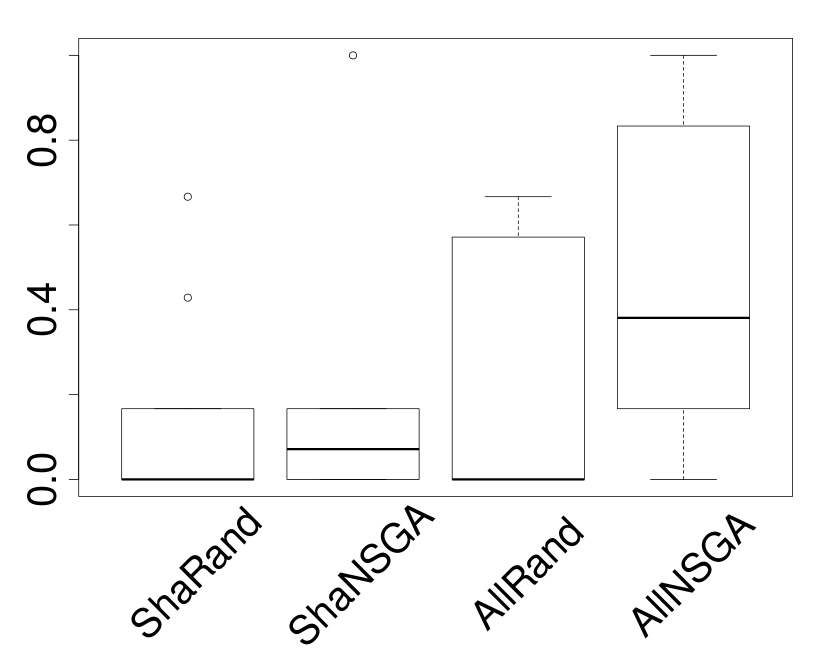
\includegraphics[width=0.22\textwidth]{sed_contribution}
	}
	\caption{Contribution indicator of \sr{}, \sn{}, \dr{}, \dn{} on all subjects. Bigger value is better.}\label{fig_contribution}
\end{figure}

\begin{figure}[htb]
	\centering
	\subfigure[espresso]{
		\label{fig_best_time_espresso}
		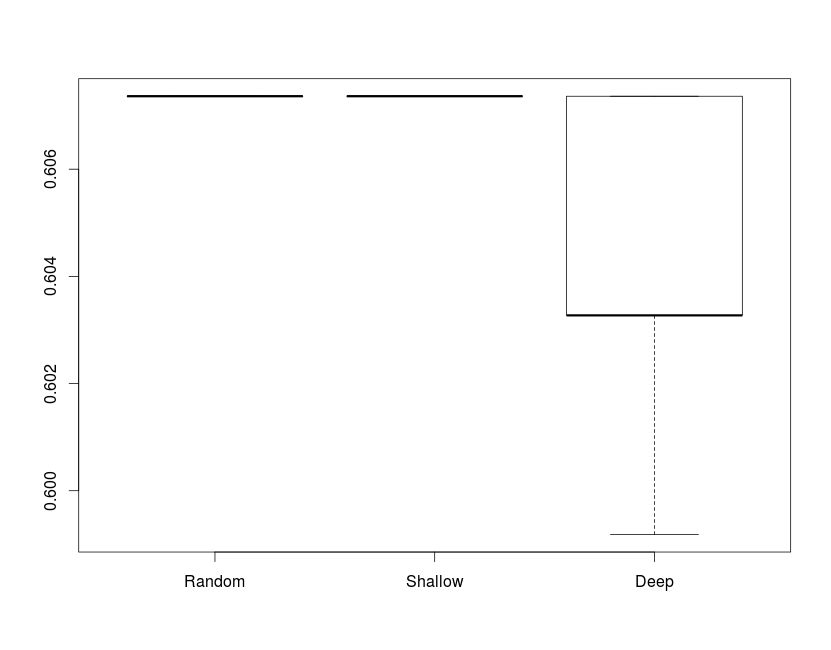
\includegraphics[width=0.22\textwidth]{espresso_best_memory}
	}
	\subfigure[gawk]{
		\label{fig_best_time_gawk}
		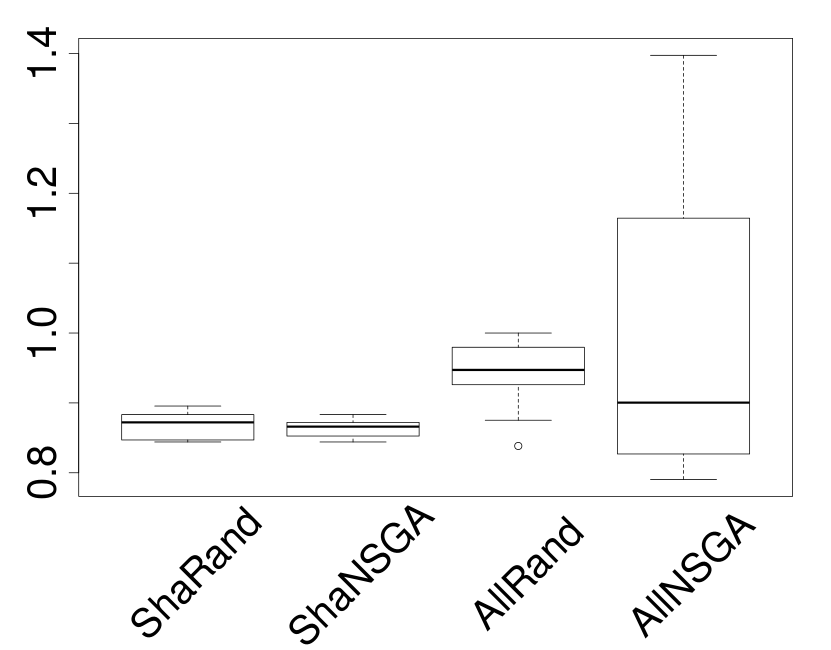
\includegraphics[width=0.22\textwidth]{gawk_best_memory}
	}
	\subfigure[flex]{
		\label{fig_best_time_flex}
		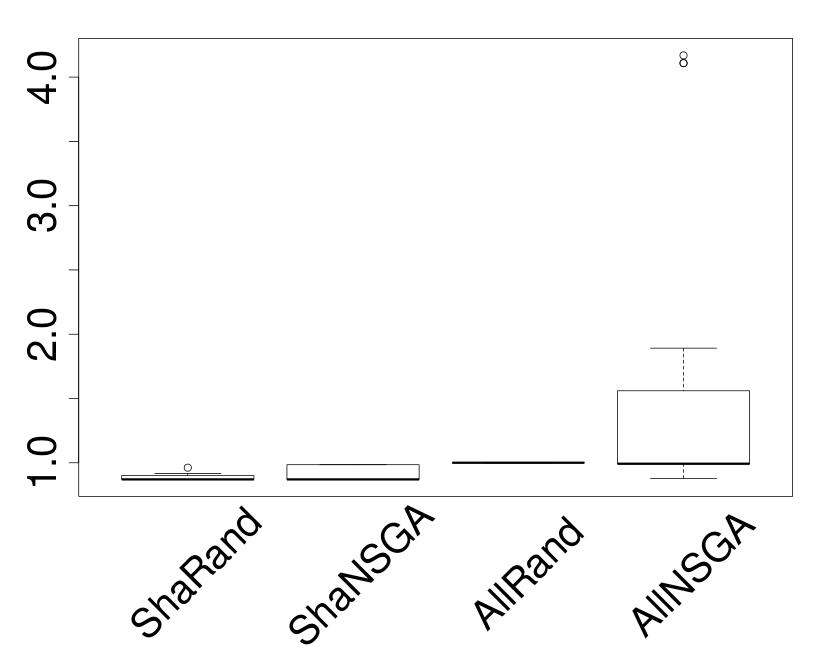
\includegraphics[width=0.22\textwidth]{flex_best_memory}
	}
	\subfigure[sed]{
		\label{fig_best_time_sed}
		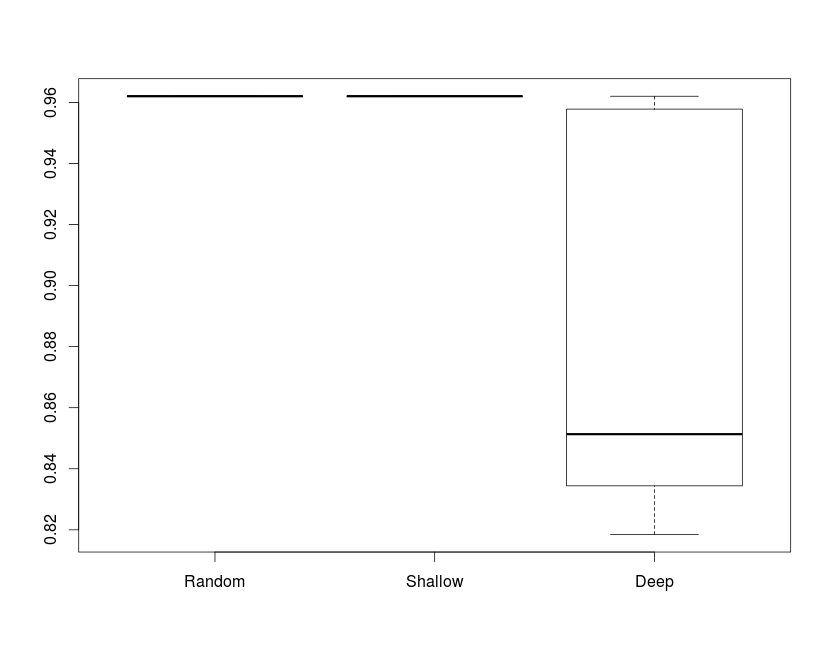
\includegraphics[width=0.22\textwidth]{sed_best_memory}
	}
	\caption{The most memory-saving performance found by each algorithm. Less is better.}\label{fig_best_memory}
\end{figure}

To have a more quantitive look at up to how much time and memory we can save from the original by our approaches, we collect the extreme performance in terms of time or memory, those have the best performance on one objective but lose a lot on the other objective, found by each algorithm on each subject and summarise them in Table \ref{table_best_time_memory}. Some of the data are too far away from the original thus not plotted in Figure \ref{fig_attainment}. 


% Please add the following required packages to your document preamble:
% \usepackage{multirow}
\begin{table*}[htbp]
\centering
\caption{Maximum reduction on time and memory for each algorithm and each subject}
\label{table_best_time_memory}
\resizebox{\textwidth}{!}{
\begin{tabular}{|c|r|r|r|r|r|r|r|r|r|r|}
\hline
\multirow{2}{*}{Subject} & \multicolumn{1}{c|}{\multirow{2}{*}{\begin{tabular}[c]{@{}c@{}}Time\\ Original (s)\end{tabular}}} & \multicolumn{4}{c|}{Time Reduction (\%)} & \multicolumn{1}{c|}{\multirow{2}{*}{\begin{tabular}[c]{@{}c@{}}Memory Original\\ (Peak/Wasted KB)\end{tabular}}} & \multicolumn{4}{c|}{Wasted Memory Reduction (\%)} \\ \cline{3-6} \cline{8-11} 
                         & \multicolumn{1}{c|}{}                                                                               & \sr{}  & \sn{}  & \dr{}  & \dn{} & \multicolumn{1}{c|}{}                                                                                            & \sr{}    & \sn{}    & \dr{}    & \dn{}    \\ \hline
espresso                 & 7.24                                                                                                & 1.4      & 1.4      & 1.5     & 1.5     & 3500/521                                                                                                         & 6.1        & 6.1        & 0          & 19.2       \\ \hline
gawk                     & 3.43                                                                                                & 3.2      & 6.7      & 4.4      & 4.4     & 29680/3552                                                                                                       & 15.6       & 15.6       & 16.2       & 20.9       \\ \hline
flex                     & 0.13                                                                                                & 4.4      & 8.9      & 6.2      & 11.6    & 10816/525                                                                                                        & 13.0       & 13.0       & 0          & 3.8        \\ \hline
sed                      & 0.25                                                                                                & 9.4      & 7.0      & 7.0      & 5.1     & 7048/948                                                                                                         & 3.8        & 3.8        & 0          & 17.9       \\ \hline
\end{tabular}
}
\end{table*}

\begin{table*}[htbp]
\centering
\caption{Computation Time}
\label{table_computation_time}
\begin{tabular}{|c|r|r|r|r|r|r|}
\hline
\multirow{2}{*}{Subject} & \multicolumn{4}{c|}{Optimisation Time (h)} & \multicolumn{1}{c|}{\multirow{2}{*}{\begin{tabular}[c]{@{}c@{}}Exposing\\ Parameters (h)\end{tabular}}} & \multicolumn{1}{c|}{\multirow{2}{*}{\begin{tabular}[c]{@{}c@{}}Extra Time Needed\\ for \dn{} from \sn{} (\%)\end{tabular}}} \\ \cline{2-5}
                         & \sr{}    & \sn{}   & \dr{}   & \dn{}   & \multicolumn{1}{c|}{}                                                                                   & \multicolumn{1}{c|}{}                                                                                                         \\ \hline
espresso                 & 39.7      & 46.4     & 9.0      & 39.3     & 12.5                                                                                                    & 18.5                                                                                                                          \\ \hline
gawk                     & 22.7      & 18.4     & 13.9     & 16.4     & 5.4                                                                                                     & 11.7                                                                                                                          \\ \hline
flex                     & 7.5       & 6.2      & 5.2      & 5.1      & 1.3                                                                                                     & 2.1                                                                                                                           \\ \hline
sed                      & 9.8       & 7.7      & 6.0      & 6.7      & 1.9                                                                                                     & 11.3                                                                                                                          \\ \hline
\end{tabular}
\end{table*}

%To answer RQ3, we manually inspect the Deep Parameters exposed from each subject program and analyse why this parameter could infect the time/memory performance of a program. There are in total 23 distinct expressions from which Deep Parameters are exposed with respect to all four subjects. Among them, five expressions are found twice by Mutation-based sensitivity analysis on two different subjects, one is found three times and two are found on all four subjects. According to our knowledge to \emph{dlmalloc}, 12 out of all 23 distinct expressions make sense that they would affect the performance if their values are changed. Moreover, 7 out of 8 expressions that are found more than once are reasonable. Due to limit space, we can only explain why the two expressions found from all subjects can affect the performance in the rest of this section.

To answer RQ3, we provide the average computation time for each of the apporaches in Table \ref{table_computation_time}. Recall that \dr{} generates and evaluates a lot of invalid configurations and each of them will crash the program and stop the evaluation immediately, the computation time of \dr{} is the lowest among all approaches. Similarly, \dn{} generates invalid configurations more often than \sn{}, so it costs less computation time than \sn{}. Taken the deep parameter exposing time into account, \dn{} costs a little more time than \sn{} does, and the percentage of the extra computation time is reported in the last column of Table \ref{table_computation_time}. According to the table, \dn{} costs at most 18\% more computation time than \sn{} (\emph{espresso}), but costs only 2\% more computation time on \emph{flex}, on which \dn{} doesn't perform as good as \sn{}. 

%The examples are shown in Figure \ref{deep_parameter}. Both of these two Deep Parameters are exposed from the function \emph{sys\_alloc()}, which manages most of the allocation from the system. The fist expression containing \emph{EXPOSE\_4334} is executed when the top chunk is not big enough to serve the memory requet and is about to be extended in system's dynamic memory, and the value of this expression decides how much memory should be get from the system this time. Smaller values tend to save memory, but may cause the program extend the top chunk more frequently, thus a waste of time. And how much memory should be get at this point may vary from applications to applications, so we expose a Deep Parameter from here so that we can control the size to be extended accordingly. The second example happens when initializing the heap. The value of the expression containing \emph{EXPOSE\_4425} is used to determine how much memory should be pre-allocated at the first time. For similar reason, bigger values tend to waste memory but save time.

